\section{Power and Energy Analysis}
\noindent
The data distribution spans from April 2020 to October 2022, showing a discrete amount of information that can be enough to make some initial observations and guessings. While there isn't a discernible pattern across the entire period, comparing plots for specific nodes (r205n01), the sum of all nodes, and individual racks reveals certain trends. \\
The lines in the plots that have a strange or unusual pattern are the result of the horizontal and vertical interpolation applied to fill some empty spaces in the distribution. No further manipulations have been applied to the data.

\vspace{-15pt}

\begin{figure}[H]
\centering
\includegraphics[width=1\textwidth]{../../PLOTS/PWR_total.png}
\captionsetup{skip=-10pt}
\caption{PWR total value (sum of all nodes in the server)}
\label{fig:PWR_total}
\end{figure}

\begin{center}
\setstretch{0.9}
count    2.110200e+04 \\
mean     7.997859e+05 \\
std      1.008300e+05 \\
min      3.101649e+04 \\
25\%      7.600741e+05 \\
50\%      8.096636e+05 \\
75\%      8.581640e+05 \\
max      1.311606e+06
\end{center}

In terms of pure power consumption, we see a visible peak that reaches a value of 1.3 MW, while the general mean stays close to 0.8 MW. The data fluctuates a lot throughout the days, but it is difficult to find any particular pattern or repetition at this level of depth; what we can guess is that all o most of the lowest points in the plot are given by a moment or period of maintenance for the server, while the highest values might indicate an episode of testing for the capabilities of the server in terms of maximum computational power.

\vspace{-15pt}

\begin{figure}[H]
\centering
\includegraphics[width=1\textwidth]{../../PLOTS/E_total.png}
\captionsetup{skip=-10pt}
\caption{E total value (sum of all nodes in the server)}
\label{fig:E_total}
\end{figure}

The energy computation was conducted based on power consumption data to derive energy values in kWh. \\
Distinct regions in the plot exhibit consistent energy levels around the mean, notably in June and August, alongside regions with negative peaks (e.g., July and October) and others with positive peaks. Understanding these peaks in the context of high-power computing offers valuable insights; \\
for example, cooling needs vary with external conditions like temperature. Peaks may coincide with hotter periods, necessitating more energy for cooling. \\
Also, changes in online service or data processing demand can influence energy consumption, e.g., heightened activity leading to increased power usage.

\subsection{PWR r205}
At rack or even node level we see a similar behaviour: a lot of peaks rising from an horizontal line that indicates the mean power consumption. 

\vspace{-15pt}

\begin{figure}[H]
\centering
\includegraphics[width=1\textwidth]{../../PLOTS/PWR_r205.png}
\captionsetup{skip=-10pt}
\caption{PWR r205}
\label{fig:PWR_r205}
\end{figure}

\vspace{-20pt}

\begin{figure}[H]
\centering
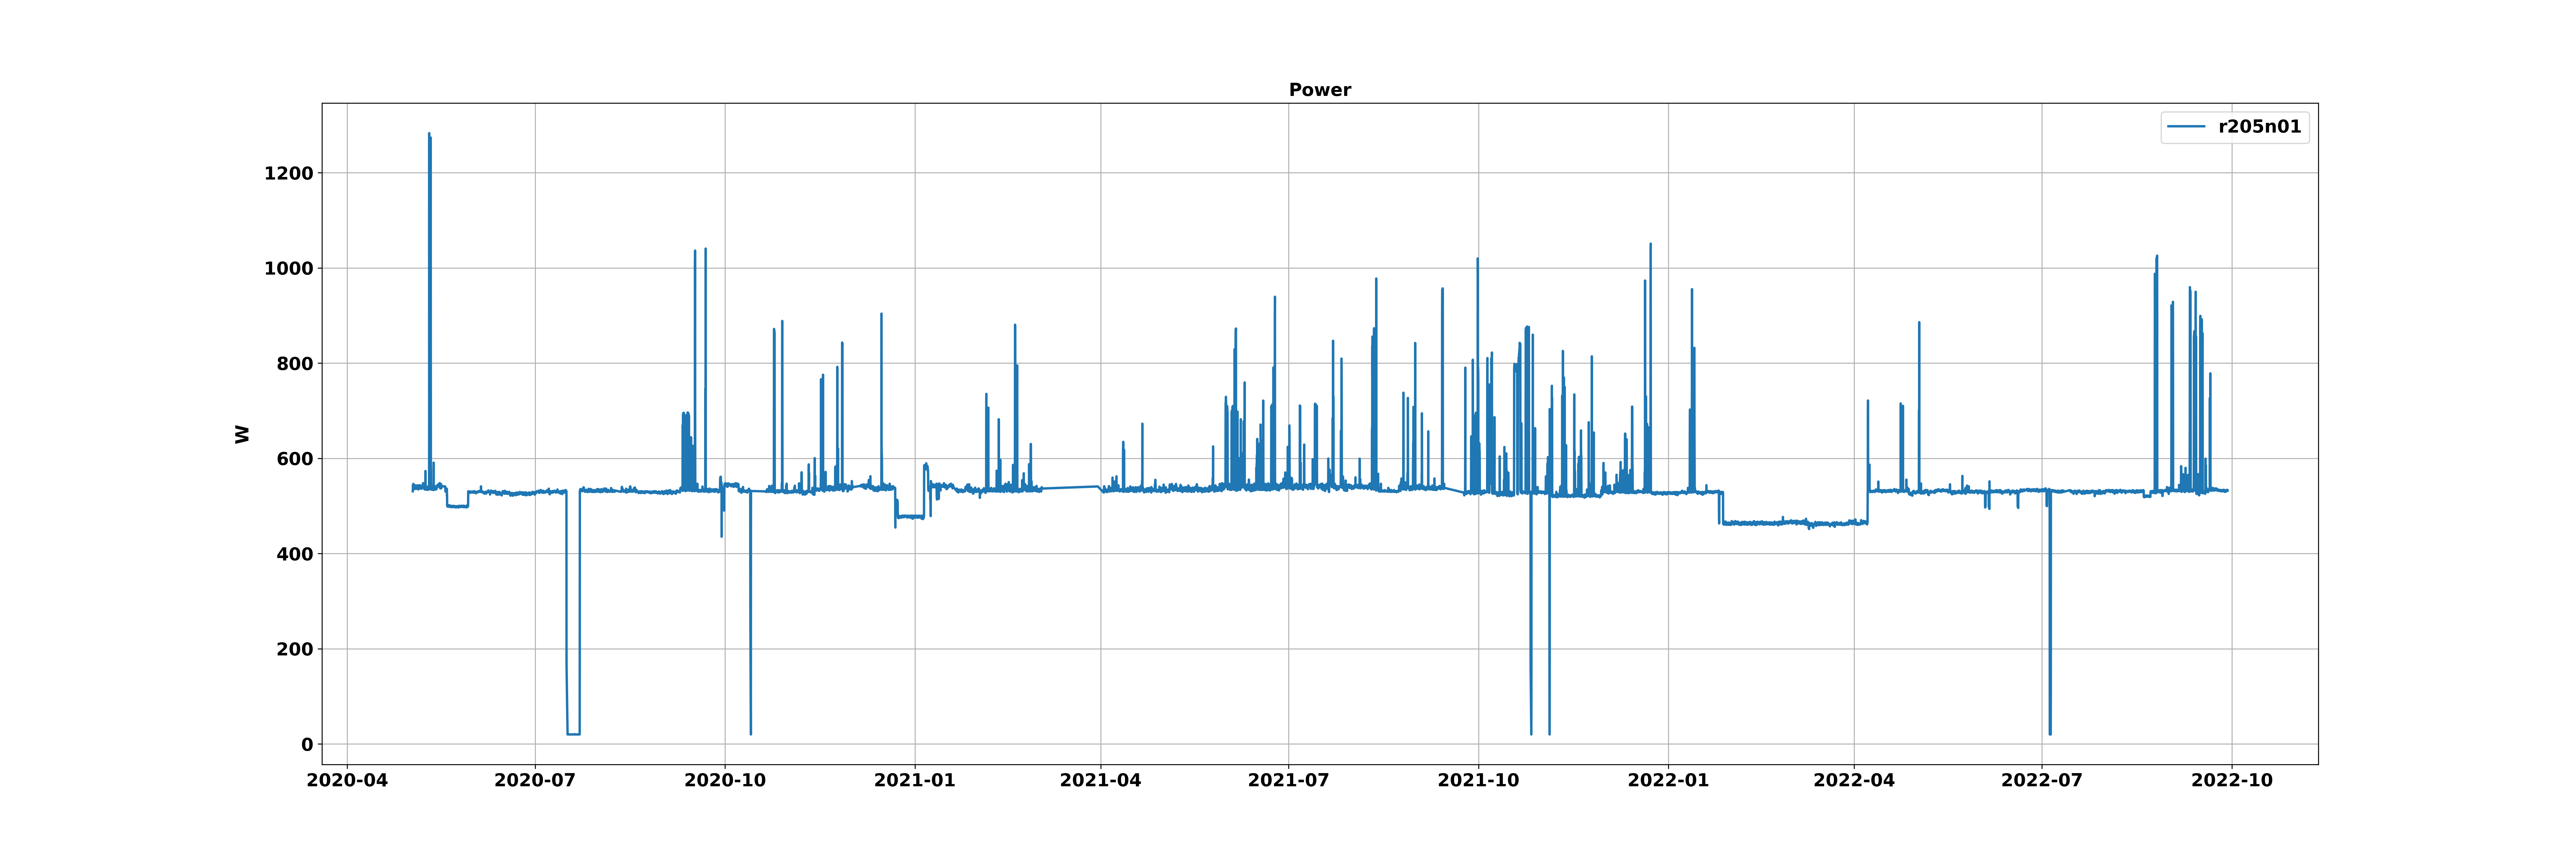
\includegraphics[width=1\textwidth]{../../PLOTS/PWR_r205n01.png}
\captionsetup{skip=-10pt}
\caption{PWR r205n01}
\label{fig:PWR_r205n01}
\end{figure}

\subsection{PWR r206}
The first rack (r205) seems to be the only one with such a regular and stable power consumption; indeed just looking at a different rack like this one (but every other rack is more similar to this) we see a much different and oscillating plot. The only hypothesis we can make is that the first rack is much less used that all the others, or maybe it is used for a different purpose.

\vspace{-12pt}

\begin{figure}[H]
\centering
\includegraphics[width=1\textwidth]{../../PLOTS/PWR_r206.png}
\captionsetup{skip=-10pt}
\caption{PWR r206}
\label{fig:PWR_r206}
\end{figure}

\vspace{-20pt}

\begin{figure}[H]
\centering
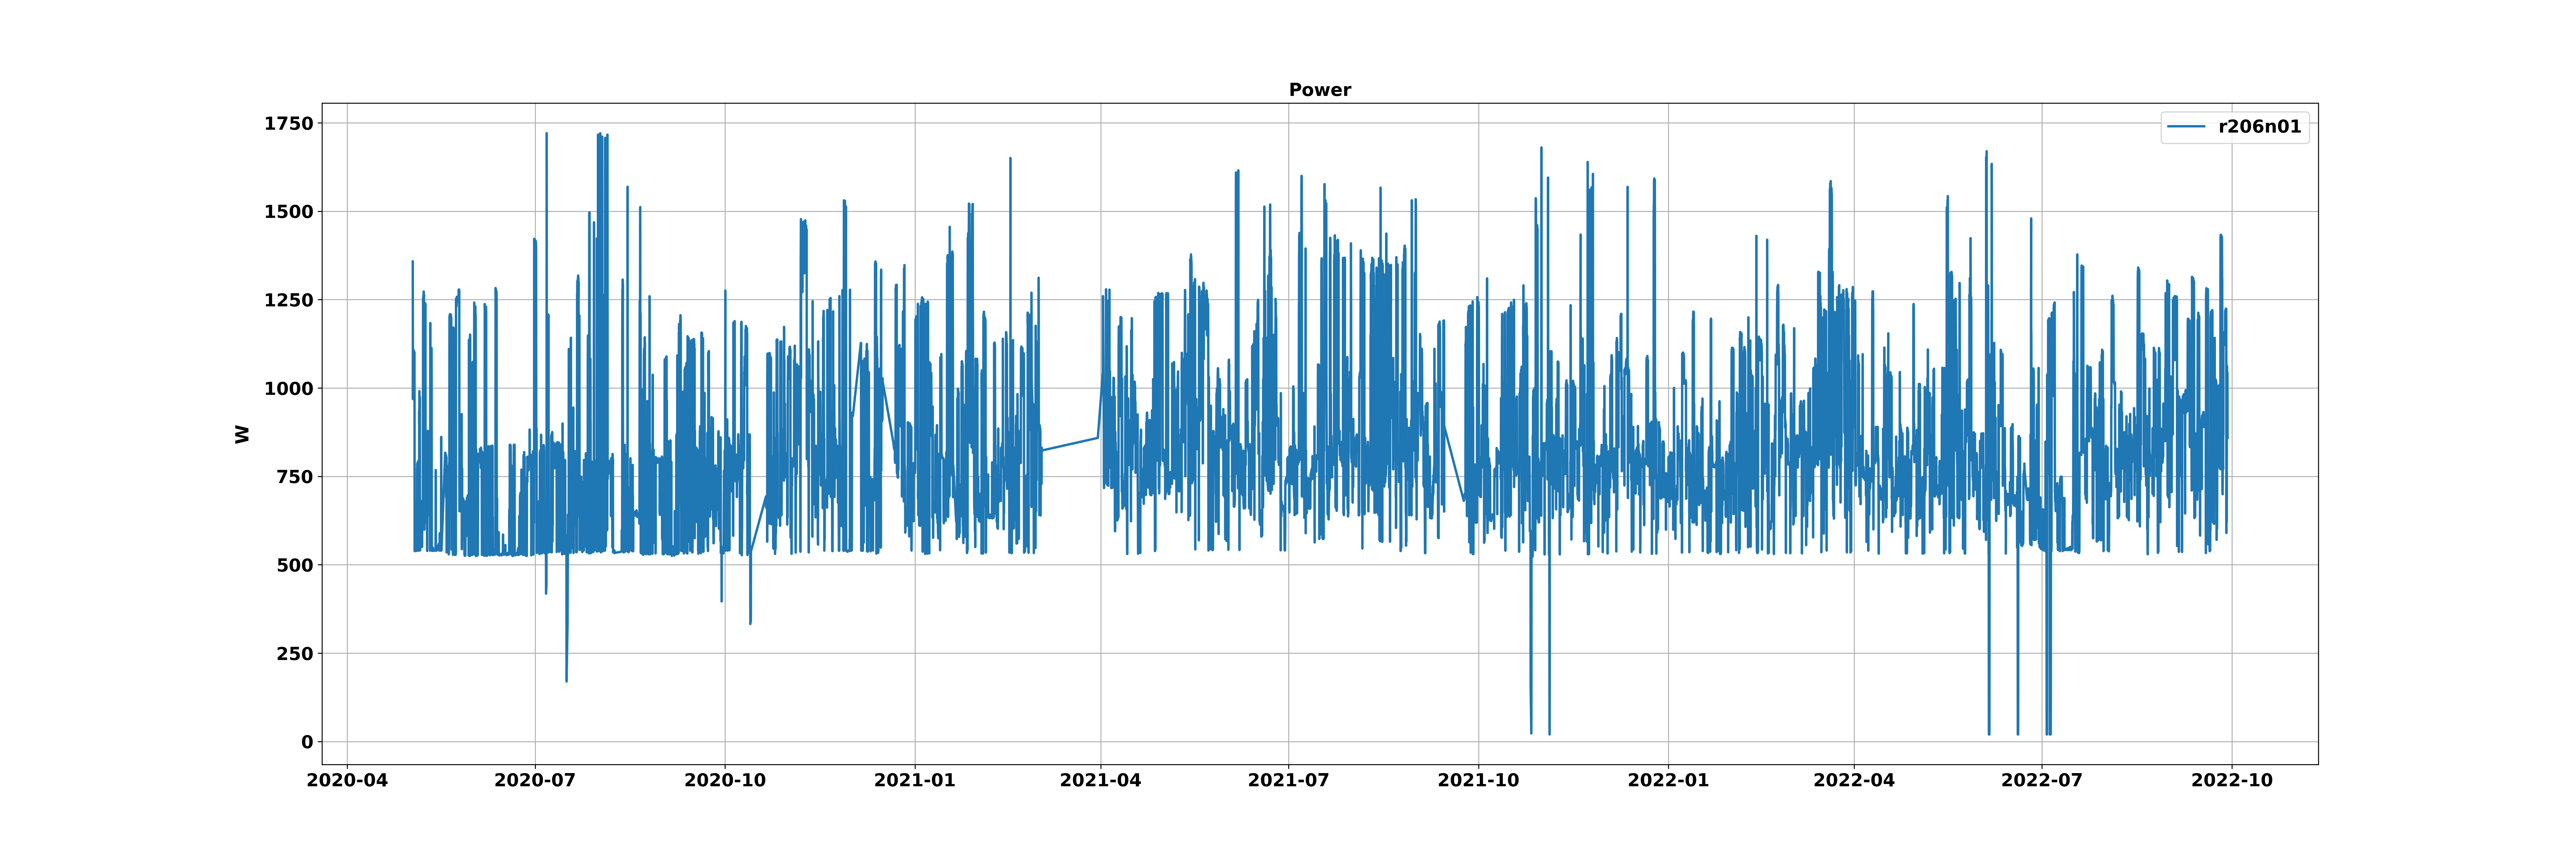
\includegraphics[width=1\textwidth]{../../PLOTS/PWR_r206n01.png}
\captionsetup{skip=-10pt}
\caption{PWR r206n01}
\label{fig:PWR_r206n01}
\end{figure}

\subsection{PWR r206n01 STL}
Even making a seasonal-trend decomposition it’s hard to highlight any specific trend, since the data is full of variations and outliers. Taking advantage of a different tool we’ll try to make any seasonality clearer.

\vspace{-10pt}

\begin{figure}[H]
\centering
\includegraphics[width=1\textwidth]{../../PLOTS/PWR_stl_r206n01.png}
\caption{PWR r206n01 STL}
\label{fig:PWR_stl_r206n01}
\end{figure}

\subsection{PWR analysis using Meta's Prophet}
Thanks to the usage of this method we are able to extract a clearer representation of the possible trends of power consumption in our server:
good choices, purely looking at the following data, might be to increase the nodes' usage during the night, during week days and also during hot seasons, all periods in which power consumption results to be lower. 

\vspace{-10pt}

\begin{figure}[H]
\centering
\includegraphics[width=1\textwidth]{../../PLOTS/PWR_prophet.png}
\caption{PWR trends}
\label{fig:PWR_prophet}
\end{figure}

Analyzing these trends aids in optimizing energy management strategies and mitigating environmental impact in high-power computing environments.
For example implementing energy optimization algorithms could reduce consumption during certain periods, resulting in negative peaks;
while aiming to a better server energy efficiency can lead to improvements in server and cooling efficiency and alter the graph's shape over time, potentially reducing energy consumption peaks.